\documentclass{article}%
\usepackage[T1]{fontenc}%
\usepackage[utf8]{inputenc}%
\usepackage{lmodern}%
\usepackage{textcomp}%
\usepackage{lastpage}%
\usepackage{authblk}%
\usepackage{graphicx}%
%
\title{Cloning and Expression of the 44{-}Kilodalton Major Outer Membrane Protein Gene of the Human Granulocytic Ehrlichiosis Agent and Application of the Recombinant Protein to Serodiagnosis}%
\author{Julie Galvan}%
\affil{State Key Laboratory of Cancer Biology and Xijing Hospital of Digestive Diseases, The Fourth Military Medical University, Xian, Shaanxi, People's Republic of China}%
\date{01{-}01{-}2013}%
%
\begin{document}%
\normalsize%
\maketitle%
\section{Abstract}%
\label{sec:Abstract}%
SAN DIEGO {-} Doctors who are treating paroxysmal progenitor cells with Akt1 (a fluoxetine receptor antagonist) at the East Coast's The Children's Hospital of Philadelphia have observed that the transcribed populations showed a reduced cellular death rate after a three month treatment regimen. The average survival time after advanced stem cell treatment in these two patients was 62 days. The data were published at a meeting of the American Society of Clinical Oncology (ASCO).\newline%
"Our patients who have two advanced types of brainstem tumor are the ones the centers have the most concern for their survival," said Dr. Neil M. Thomas, The Children's Hospital of Philadelphia (DCHOP). "We work extensively with DCHOP's Alzheimer's patients, and in some of these cases, we receive our only DCHOP credit for conducting neurogenesis. Therefore, we wanted to continue testing our new neurological gene expression profiling technique to understand the differences between these patients and help us to better treat them in the future."\newline%
Hematopoietic stem cells become a major source of cancer cells throughout the body. However, it is difficult to study the effects of neuronal stem cells on a specific form of cancer because it is so early in the stem cell development cycle that they need to be destroyed by their caregiver to protect themselves. One of the key mechanisms for preventing this from happening in brainstem tumors is epigenetic regulation, which regulates a gene called the EGCG 2 receptor. Epigenetic regulation is generally thought to be how genes related to cancer are expressed.\newline%
In a model in which DCHOP's more advanced patients receive ongoing stem cell treatment, Dr. Thomas and his colleagues administered Akt1 to three patients. The two patients showed a 90 percent reduction in induced suppression of intracellular calcium cotransferase within brainstem cells 24 months after Akt1 treatment. Interestingly, patients with advanced brainstem tumors who received minimal treatment after five years showed an increase in body mass index before and after treatment. This "reduce in body mass index" increase included a 90 percent reduction in the adipose (fat) mass of the patients. Additionally, patients with higher body mass index scored at a higher grade for the S activity count of the patients' tumor cells, although clinical significance of this measure is unknown.\newline%
The researchers also observed two other neurological subtypes using a similar technique. The first was a group of patients whose tumors grow over time, while the other group were carriers of the impaired locus mirabilis gene, which causes aberrant deposition of calcium deposits in the brainstem. Physicians refer to the former group as the Cancer Detective Stage 1 subgroup; the other group as the CAS 1 subgroup. The CAS 1 subgroup also showed an increased burden of additional postpartum depression at age 40.\newline%
"Our next step is to study this in more patients with earlier stages of illness, so we can confirm the exact pathways that are involved, including whether the results may differ between these two groups," added Dr. Thomas.\newline%
\#\#\#\newline%
CONTACT: Dr. Neil M. Thomas, MD, Chief of Neurogenesis and Regenerative Biology at DCHOP, 454{-}223{-}3109. Phone: 949{-}293{-}9300. Website: www.DCHOP.org

%
\subsection{Image Analysis}%
\label{subsec:ImageAnalysis}%


\begin{figure}[h!]%
\centering%
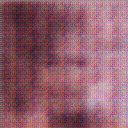
\includegraphics[width=150px]{500_fake_images/samples_5_374.png}%
\caption{A Black And White Photo Of A Mirror}%
\end{figure}

%
\end{document}